% !TEX root = ../dissertation.tex

\chapter{Introduction}
\label{chapter:introduction}

\section{Motivation}

Game playing has always been a fundamental part of Artificial Intelligence (AI) research, as it can be used to test strategy in a straightforward way. Different games can be created to test specific features or properties that are of research interest, such as opponent modeling.

Throughout the history of AI research there was always a big focus on the ability of playing specific games, like chess, well. This focus led to systems like Deep Blue (the computer system that defeated Garry Kasparov at chess in the 90’s) that, while very advanced on the games they are designed for, delegate all the interesting analysis to the system designers. These systems are also completely useless for all games other than the one they were designed for (even if the difference is very small).

This over-specialization limits the usefulness of these systems. It is then of our interest to also be able to design more general systems, which could be closer to one of the most powerful features of human intelligence, adaptability:

\chapquote{``A human being should be able to (...) design a building, write a sonnet, balance accounts, build a wall, set a bone, comfort the dying, take orders, give orders, cooperate, act alone, solve equations, analyze a problem, pitch manure, program a computer, fight efficiently, die gallantly. \\ Specialization is for insects.''}{Robert A. Heinlein}{Time Enough for Love}

\gls{GGP} aims to develop general game playing systems, systems that can play any game when given the rules, acting as a stepping stone for General Intelligence research. Artificial General Intelligence has been a topic for science-fiction stories and, if possible, can be the biggest revolution in human history, allowing for an unprecedented ability of problem-solving.

\section{Multi-game playing}

Multi-game playing is the concept of developing programs that can play not just one, but many different games. This is not to be mistaken with combining many programs into one, multi-game players should be able to adapt to games unknown to them as well. Doing this requires many traits shared by \textit{Artificial Intelligence} research, such as deduction, reasoning, problem solving, intelligent search, knowledge representation, planning and learning.

General Game Playing was proposed in 2005 by Standford University as a platform for for multi-game playing research, along with a language for describing games, the \gls{GDL}. An online course was created by Standford University and there are several new GGP projects every year, as well as various competitions, the biggest one being the annual GGP competition, held at the AAAI conference.

More recently another platform also appeared, General Video-Game Playing (GGVP), which focuses on video games.

\subsection{Early attempts at multi-game playing}

Possibly the earliest work on the subject was done in 1969 in \cite{Pitrat1969}. There were other notable works in the 90's, like SAL, Hoyle, Morph, METAGAMER (all sumarized in \cite{Mandziuk2013}) and Zillions of Games. Hoyle is described in more detail below.

\subsubsection{Hoyle}
A system developed in the 90’s, using a training scheme called lesson and practice, where lessons are games played against an expert and practice is self-playing. Predates GDP and was developed for 2-player games. The system used a set of game independent Advisers, each specialized in a game aspect such as position. These Advisers could recommend moves that could then be chosen by higher tier advisers. There were 3-tiers, depending on specialization:

\begin{enumerate}

\item [1st.] These Advisers specialized in immediate consequences: they performed very shallow searches to avoid things like instant loss moves. These decisions were final.

\item [2nd.] Advisers in this tier chose moves according to certain goals. These decisions were also final.

\item [3rd.] Advisers in the last tier differed from the first tiers in an important way: The decision of each Adviser wasn’t final, the final decision was decided by a process similar to taking a vote between the Advisers in this 3rd tier. Advisers votes were weighted in accordance to the lesson and practice results: Advisers that were more often correct during the training stage received bigger weights.

\end{enumerate}
This process of weighting the Advisers was crucial to the performance of the system and could even be worse than a random player if done incorrectly. If none of the 3rd tier advisers were even remotely related to the game being played the results would also be disappointing. Having a varied pool of Advisers was for this reason vital but they were never, by definition, general enough to be useful for any game. Hoyle was tested in 18 two-player board games, its potential in complex games was never verified.


\section{Objectives}

\paragraph{Main Objectives:}
\begin{itemize}
\item Research and compare current techniques and solutions for GGP players
\item Improve or develop new techniques for game playing
\item Use the improvements to make a new GGP player
\item Benchmark the player against other existing GGP players
\end{itemize}

\paragraph{Secondary Objectives:}
\begin{itemize}
\item Publish the results
\item Take the online course on GGP
\item Enter the annual GGP competition
\item Enter other relevant competitions
\end{itemize}




\section{Planning}


\begin{table}[h]
\caption{Expected dates for the dissertation objectives}
\label{table:Planning}
\small
%\begin{tabular}{| c | p{1cm} | p{2.5cm} | p{2.5cm} | p{2.8cm} | c | p{2.2cm} |}
\begin{tabular}{| c | c | c |}
\hline Objective & Start date & End date \\

\hline Research and compare current techniques and solutions for GGP players & 18/Jan/2016 & 14/Feb/2016 \\
\hline Improve or develop new techniques for game playing & 01/Feb/2016 & 10/Apr/2016 \\
\hline Use the improvements to make a new GGP player & 11/Apr/2016 & 22/May/2016 \\
\hline Benchmark the player against other existing GGP players & 23/May/2016 & 12/Jun/2016 \\

\hline \\

\hline Publish the results & 20/Jun/2016 & 17/Jul/2016 \\
\hline Take the online course on GGP & 28/Mar/2016 & 17/Jul/2016 \\
\hline Enter the annual GGP competition & 06/Jun/2016 & 15/Jun/2016 \\
\hline Enter other relevant competitions & - & - \\

\hline
\end{tabular}
\end{table}


\begin{figure}[h]
	\centering
    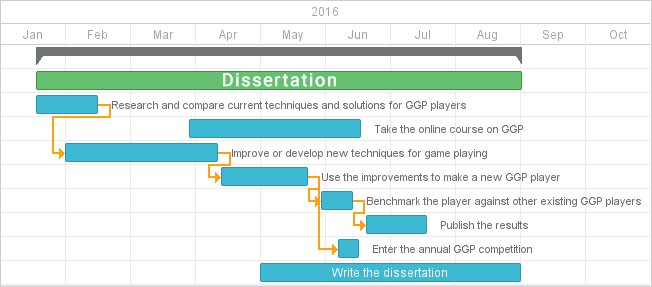
\includegraphics[scale=0.6]{images/gantt.png}
    \caption{Gantt chart for the dissertation}
    \label{fig:gantt}
\end{figure}

% A demonstration of how to use acronyms and glossary:

% A \gls{MSc} entry.

% Second use: \gls{IST}.

% Plurals: \glspl{MSc}.

% A citation example \cite{nobody}
